\chapter{XÂY DỰNG MẠNG NHẬN DẠNG NGÔN NGỮ KÝ HIỆU TỪ TỌA ĐỘ KHUNG XƯƠNG}
\label{s:DNN}
Trong chương 3, thuật toán ước tính tư thế khung xương đã được trình bày chi tiết về lý thuyết và phương pháp xử lý áp dụng thuật toán. Ta thấy rằng phương pháp này hỗ trợ rất tốt cho việc ước tính nh anhtư thế khung xương trong xử lý thời gian thực. Trong chương 4 này, luận văn sẽ trình bày về đề xuất mô hình mạng DNN lấy đầu vào là toạ độ khung xương được ước tính và nhận dạng cử chỉ thời gian thực. Nội dụng chương trình bày cấu trúc mạng neural network đề xuất, cách thu thập và xử lý dữ liệu cũng như sơ đồ hoạt động chương trinh.
\section{Tổng quan}
Một hành động của con người được đánh giá, xem xét bằng một loạt các cử chỉ theo thời gian. Tuy nhiên, khi xem xét các hành động của con người nhằm tìm ra một cấu trúc nhất quán và có thể tạo thành mô hình thì gặp các vấn đề phức tạp sau:

$\bullet$ Nếu chỉ xem xét đường bao của con người, các phần cơ thể của con người quá gần nhau để có thể xác định được chính xác phần cơ thể cần thiết.

$\bullet$ Hình dạng của cử chỉ (đường bao con người, màu sắc các phần cơ thể), vị trí, loại và kiểu của cử chỉ rất phức tạp. Việc xem xét một mô hình có thể biểu diễn toàn bộ các hành động ngôn ngữ ký hiệu hầu như không thể xem xét nên trong phạm vi luận văn này chỉ xem xét đến việc một mô hình có thể biểu diễn 16 cử chỉ cần sự phối hợp cả hai tay và các cử chỉ tương đối khác nhau (\textbf{Xin chào, Tôi, thành phố, vui vẻ, ẵm em, Sài Gòn, Vĩnh Long, đi bộ, mùa màng, đói bụng, yêu, ăn, biểu quyết, đứng yên, hẹp, rộng}).

$\bullet$ Các hành động của con người có thể giống nhau, tuy nhiên nếu việc quan sát hoặc camera quan sát nằm ở vị trí khác nhau, hướng, độ cao,... đều ảnh hưởng đến khả năng nhận diện hành động của con người. Luận văn đã nêu được phương pháp để có thể phát triển cho việc xác định hành động của con người khi vị trí của camera thay đổi. Tuy nhiên việc kiểm chứng khả năng hoạt động ở các vị trí camera khác nhau sẽ được xem xét ở tương lai.

$\bullet$ Nếu một phần cơ thể bị che khuất bởi các vật thể thì việc xác định hành động của con người sẽ gặp khó khăn hơn rất nhiều so với trường hợp không bị che khuất, phạm vi luận văn không xem xét đến vấn đề này. Tuy nhiên đây là một điểm cần xem xét đến để có thể hoàn thiện hệ thống nhận diện cử chỉ trong tương lai.
\section{Thu thập dữ liệu}
Dữ liệu đầu vào là tọa độ của 18 khớp xương được detect từ mạng mobilenet. Các khớp xương được xuất ra từ mạng được đánh số thứ tự từ 0 tới 17. Các khớp xương cụ thể được thể hiện trong bảng \ref{table:joints} và trong hình \ref{fig:joints}.


\begin{table}[h]
\caption{Các khớp xương được xuất ra từ mạng}
\label{table:joints}
\centering
\begin{center}
\begin{tabular}{|c|p{9cm}|} 
 \hline
Số thứ tự khớp xương  & Vị trí \\
 \hline
 0 & Mũi\\
 \hline 
 1 & Cổ\\
 \hline 
 2 & Vai phải\\
 \hline
 3 & Khủy tay phải \\
 \hline 
 4 & Cổ tay phải\\
 \hline
 5 & Vai trái\\
 \hline
 6 & Khủy trái\\
 \hline
 7 & Cổ tay trái\\
 \hline
 8 & Hông phải\\
 \hline
 9 & Đầu gối phải\\
 \hline
 10 & Cổ chân phải\\
 \hline
 11 & Hông trái\\
 \hline
 12 & Đầu gối trái\\
 \hline
 13 & Cổ chân trái\\
 \hline
 14 & Mắt phải\\
 \hline
 15 & Mắt trái\\
 \hline
 16 & Tai phải\\
 \hline
 17 & Tai trái\\
 \hline
\end{tabular}
\end{center}
\end{table}

Đầu tiên người thu thập dữ liệu đứng trước camera, thực hiện hành động thể hiện từ cần huấn luyện. Chương trình thu thập dữ liệu sẽ xuất ra tọa độ khung xương sau khi xử lý qua mạng pose estimate. Sau đó lưu các tọa độ khớp xương cùng với nhãn của hành động vào file "data.csv" để sau đó đưa vào train. Hình \ref{fig:joints} thể hiện quá trình khi thu thập dữ liệu.


\FloatBarrier
\begin{figure}[htp]
\begin{center}
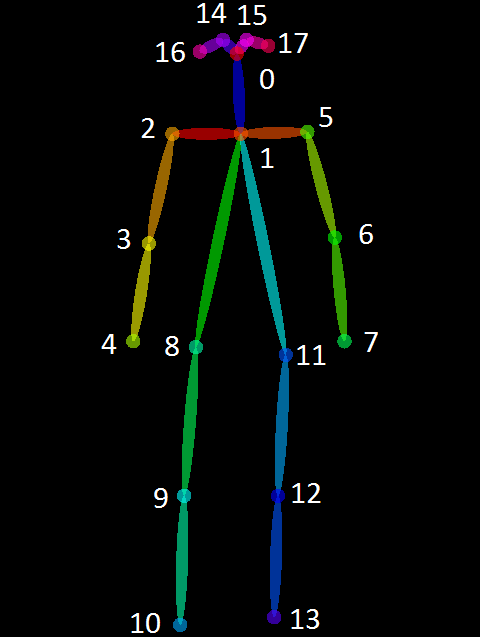
\includegraphics[scale=0.6]{chap4/c4_figs/joints_order.png}
\end{center}
\caption{Sơ đồ khớp xương xuất ra từ mạng mobilenet}
\label{fig:joints}
\end{figure}
\FloatBarrier

\section{Xử lý dữ liệu đầu vào}
Dữ liệu sau khi thu thập ban đầu bao gồm tất cả tọa độ các khớp xương ứng các hành động cần nhận dạng. Tuy nhiên khi huấn luyện bộ nhận diện ngôn ngữ ký hiệu ta cần phải xử lý lại dữ liệu khớp xương đã thu thập được. Quá trình xử lý trải qua 2 phần: Loại bỏ các phần khớp xương dư thừa, sau đó chuẩn hóa lại các vector SJM.

\subsection{Loại bỏ các phần SJM dư thừa}
Ngôn ngữ ký hiệu với đặc trưng là sự phối hợp phần trên cơ thể với hai tay để diễn đạt từ ngữ mong muốn. Do đó việc xem xét đến các khớp xương phần dưới cơ thể là không cần thiết. Phần xử lý này, đề tài đã loại bỏ các tọa độ SJM dư thừa, chỉ giữ lại 10 điểm khớp xương cần thiết cho việc nhận diện: \textbf{Mũi, Cổ, Vai trái, khuỷu tay trái, Cổ tay trái, Vai phải, Khủy tay phải, Cổ tay phải, hông phải và hông trái} như thể hiện trong hình \ref{fig:joints} và bảng \ref{table:joints_choose}

\FloatBarrier
\begin{figure}[htp]
\begin{center}
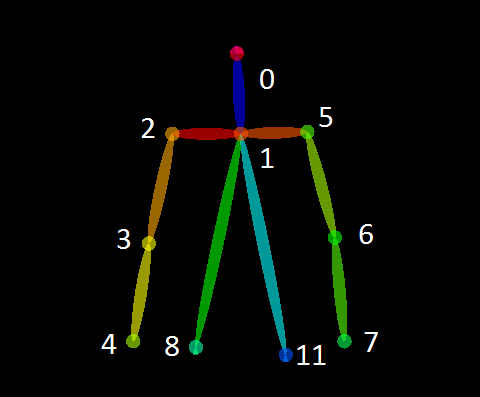
\includegraphics[scale=1]{chap4/c4_figs/joints_choose.png}
\end{center}
\caption{Sơ đồ khớp xương sau khi loại bỏ các phần không cần thiết}
\label{fig:joints}
\end{figure}
\FloatBarrier

\FloatBarrier
\begin{table}[h]
\caption{Các khớp xương được giữ lại}
\label{table:joints_choose}
\centering
\begin{center}
\begin{tabular}{|c|p{9cm}|} 
 \hline
Số thứ tự khớp xương  & Vị trí \\
 \hline
 0 & Mũi\\
 \hline 
 1 & Cổ\\
 \hline 
 2 & Vai phải\\
 \hline
 3 & Khủy tay phải \\
 \hline 
 4 & Cổ tay phải\\
 \hline
 5 & Vai trái\\
 \hline
 6 & Khủy trái\\
 \hline
 7 & Cổ tay trái\\
 \hline
 8 & Hông phải\\
 \hline
 11 & Hông trái\\
 \hline
\end{tabular}
\end{center}
\end{table}
\FloatBarrier

\subsection{Chuẩn hóa SJM để phân loại đặc trưng}

Dựa vào dữ liệu thu thập được, ta có thể nhận thấy là tùy vào vị trí camera, khoảng cách từ camera đến người được quan sát sẽ làm thay đổi giá trị của các vector khung xương SJM. Hình \ref{fig:skeleton} ta có thể thấy khoảng cách các vector tọa độ khung xương của người ở xa camera sẽ gần nhau hơn so với người ở gần. Do đó cần phải sử dụng phương pháp chuẩn hóa dữ liệu các vector, đưa các vector đặc trưng SJM về cùng kích cỡ thì dữ liệu đưa vào train mới có thể có cùng những đặc trưng giống nhau.

Phương pháp chuẩn hóa được áp dụng như sau:
...
...




Sau khi loại bỏ các phần thừa và chuẩn hóa hết bộ dữ liệu các SJM, ta được các SJM với tọa độ các điểm khớp xương được chuẩn hóa nằm trong khoảng 0 --> 1 thể hiện trong hình \ref{fig:skeleton_normalize}
\FloatBarrier
\begin{figure}[htp]
\begin{center}
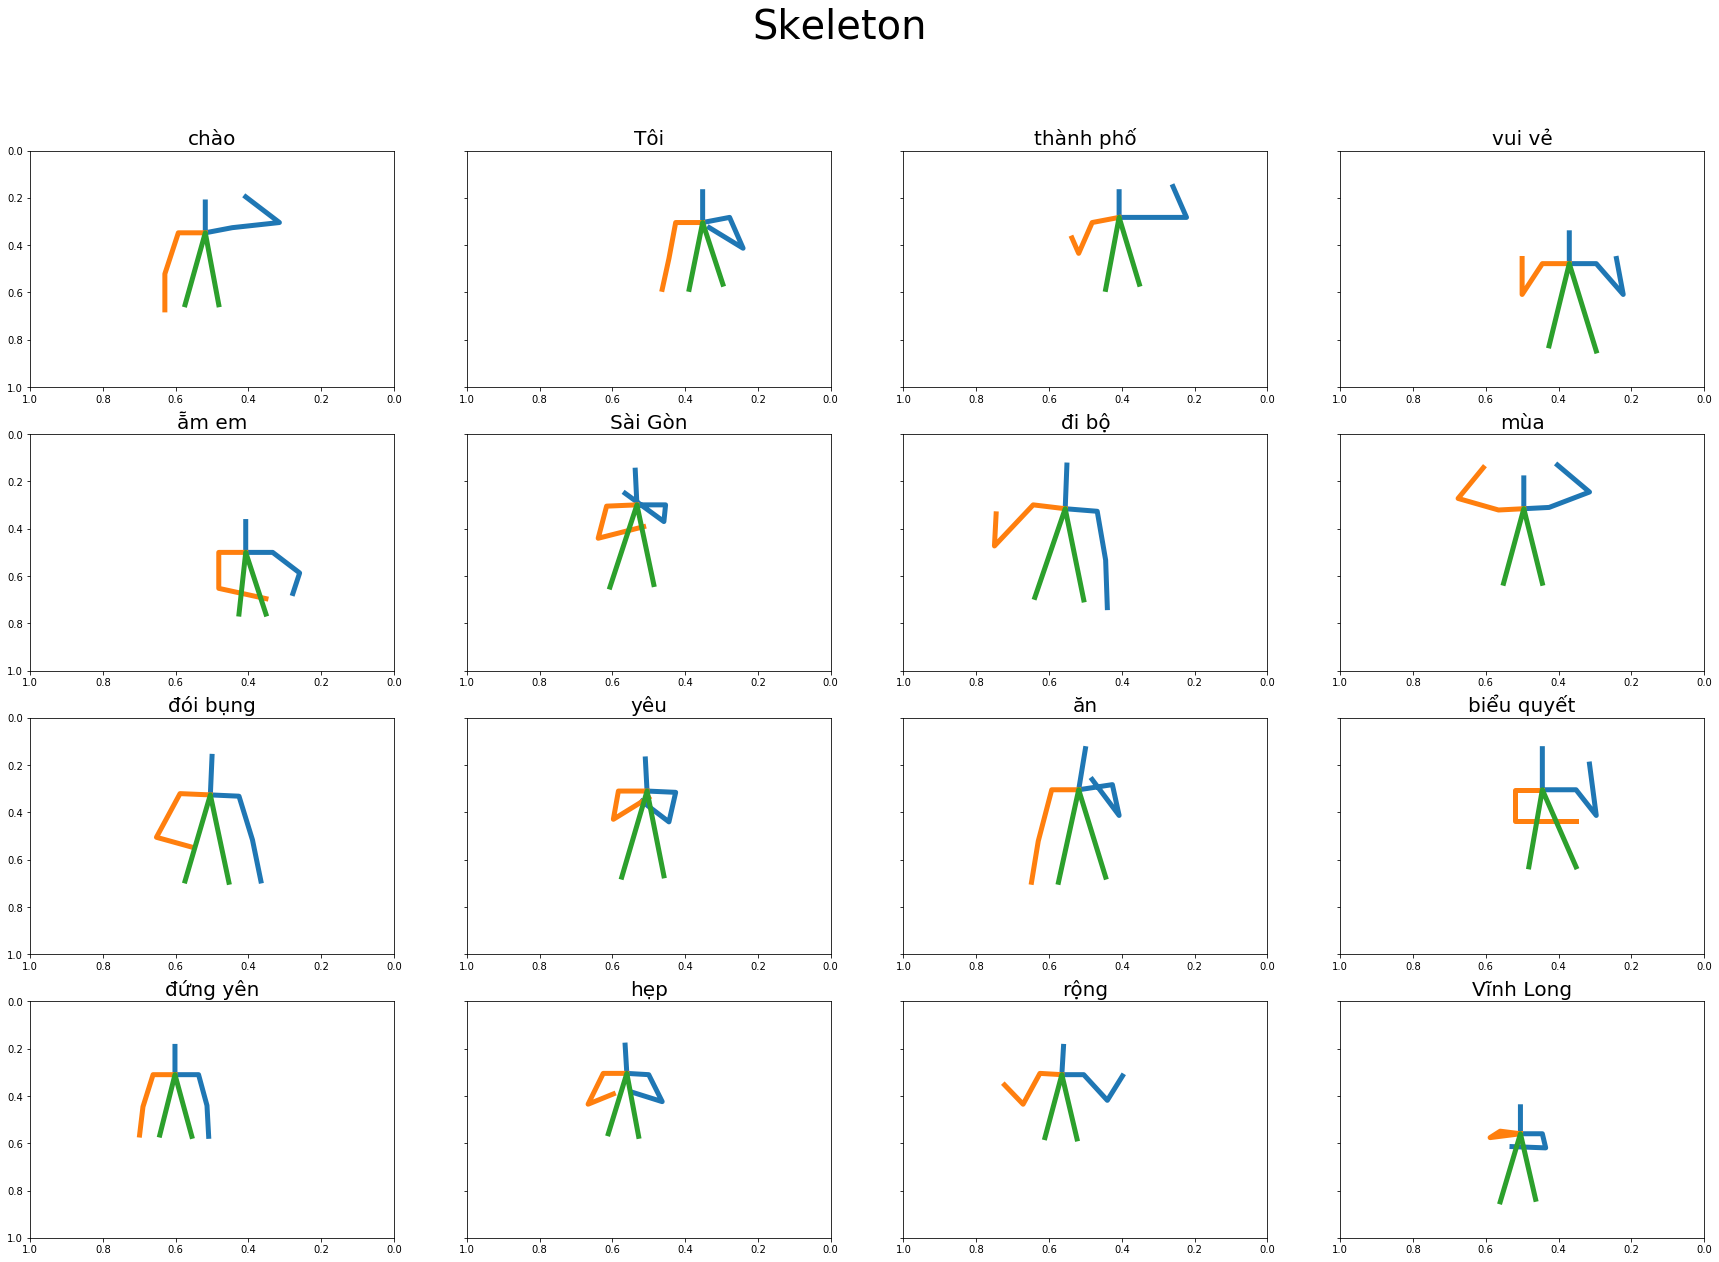
\includegraphics[scale=0.25]{chap4/c4_figs/datajoint.png}
\end{center}
\caption{Dữ liệu khớp xương sau khi đã được chuẩn hóa}
\label{fig:skeleton_normalize}
\end{figure}
\FloatBarrier

\section{Cấu trúc mạng neural network đề xuất}
Từ dữ liệu đầu vào là một ảnh RGB, qua bước phát hiện khung xương với mạng CNN và các bước chuẩn hóa, loại bỏ khớp xương thừa, dữ liệu cần phân loại gần như đã lấy ra hết đặc trưng cần tìm và giảm số chiều đến tối đa. Do đó mạng DNN cần dùng để phân loại các từ ngôn ngữ ký hiệu chỉ cần một cấu trúc vừa phải và giảm thiểu số trọng số đến tối đa.
\begin{itemize}
\item Input: Mạng với đầu vào là 20 nodes ứng với tọa độ của 10 khớp xương (mỗi khớp là 2 tọa độ).
\item Hidden layer: Là các lớp Fully connected (Dense) và Normalization xen kẽ nhau.
\item Output: Với softmax với 16 nodes ứng với 16 từ ngữ nhận diện được.
\end{itemize}
Cụ thể các thông số và cấu trúc được thể hiện trong hình \ref{fig:model_params} và \ref{fig:model}.

\FloatBarrier
\begin{figure}[htp]
\begin{center}
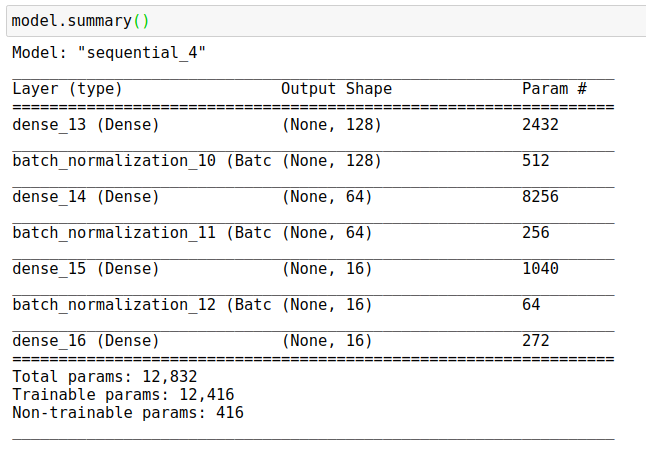
\includegraphics[scale=1.3]{chap4/c4_figs/model_param.png}
\end{center}
\caption{Các thông số của mạng DNN}
\label{fig:model_params}
\end{figure}
\FloatBarrier

\FloatBarrier
\begin{figure}[htp]
\begin{center}
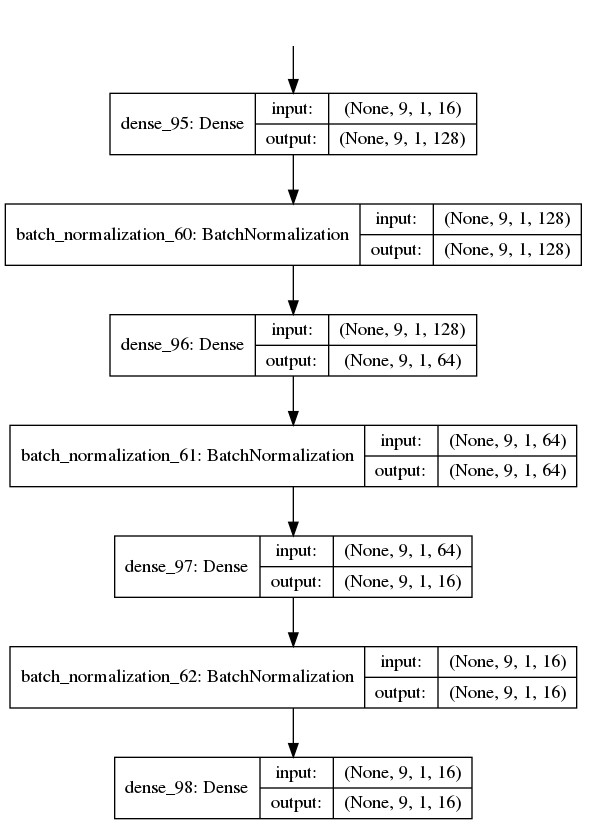
\includegraphics[scale=0.9]{chap4/c4_figs/model.png}
\end{center}
\caption{Cấu trúc mạng sau khi được vẽ bằng thư viện keras}
\label{fig:model}
\end{figure}
\FloatBarrier

Model sử dụng khá nhiều lớp Batch Normalization. Về lý thuyết toán thì layer này có tác dụng trong 2 việc đó là:
\begin{itemize}
\item Tránh gradient tiến về 0 sẽ chẳng biết là đi lên hay xuống.
\item Gradient quá lớn khiến các tham số không thể tối ưu được (loss sẽ nhảy lung tùng).
\end{itemize}
Cụ thể là nó giúp chuẩn hóa dữ liệu về 1 khoảng nào đó ví dụ (0,1).

\section{Huấn luyện mạng}
Mạng được huấn luyện theo thuật toán Stochastic Gradient Descent (SGD) là một biến thể của Gradient Descent. Cụ thể ta sẽ tìm hiểu về nó qua các phần dưới dây.

\subsection{Gradient Descent}
Trong Machine Learning nói riêng và Toán Tối Ưu nói chung, chúng ta thường xuyên phải tìm giá trị nhỏ nhất (hoặc đôi khi là lớn nhất) của một hàm số nào đó. Ví dụ như các hàm mất mát trong hai bài Linear Regression và K-means Clustering. Nhìn chung, việc tìm global minimum của các hàm mất mát trong Machine Learning là rất phức tạp, thậm chí là bất khả thi. Thay vào đó, người ta thường cố gắng tìm các điểm local minimum, và ở một mức độ nào đó, coi đó là nghiệm cần tìm của bài toán.

Các điểm local minimum là nghiệm của phương trình đạo hàm bằng 0. Nếu bằng một cách nào đó có thể tìm được toàn bộ (hữu hạn) các điểm cực tiểu, ta chỉ cần thay từng điểm local minimum đó vào hàm số rồi tìm điểm làm cho hàm có giá trị nhỏ nhất. Tuy nhiên, trong hầu hết các trường hợp, việc giải phương trình đạo hàm bằng 0 là bất khả thi. Nguyên nhân có thể đến từ sự phức tạp của dạng của đạo hàm, từ việc các điểm dữ liệu có số chiều lớn, hoặc từ việc có quá nhiều điểm dữ liệu.

Hướng tiếp cận phổ biến nhất là xuất phát từ một điểm mà chúng ta coi là gần với nghiệm của bài toán, sau đó dùng một phép toán lặp để tiến dần đến điểm cần tìm, tức đến khi đạo hàm gần với 0. Gradient Descent (viết gọn là GD) và các biến thể của nó là một trong những phương pháp được dùng nhiều nhất.

Các bước quan trọng của thuật toán Gradient Descent như sau:
\begin{itemize}
\item Dự đoán một điểm khởi tạo $\theta = \theta_0$.
\item Cập nhật $\theta$ đến khi đạt được kết quả chấp nhận được: 
$$\theta = \theta - \eta \nabla_{\theta}J(\theta)$$
với $\nabla_{\theta}J(\theta)$ là đạo hàm của hàm mất mát tại $\theta$
\end{itemize}

\textbf{Gradient dưới góc nhìn vật lý:}

Thuật toán GD thường được ví với tác dụng của trọng lực lên một hòn bi đặt trên một mặt có dạng như hình một thung lũng giống như hình \ref{fig:gradient} dưới đây. Bất kể ta đặt hòn bi ở A hay B thì cuối cùng hòn bi cũng sẽ lăn xuống và kết thúc ở vị trí C.

\FloatBarrier
\begin{figure}[htp]
\begin{center}
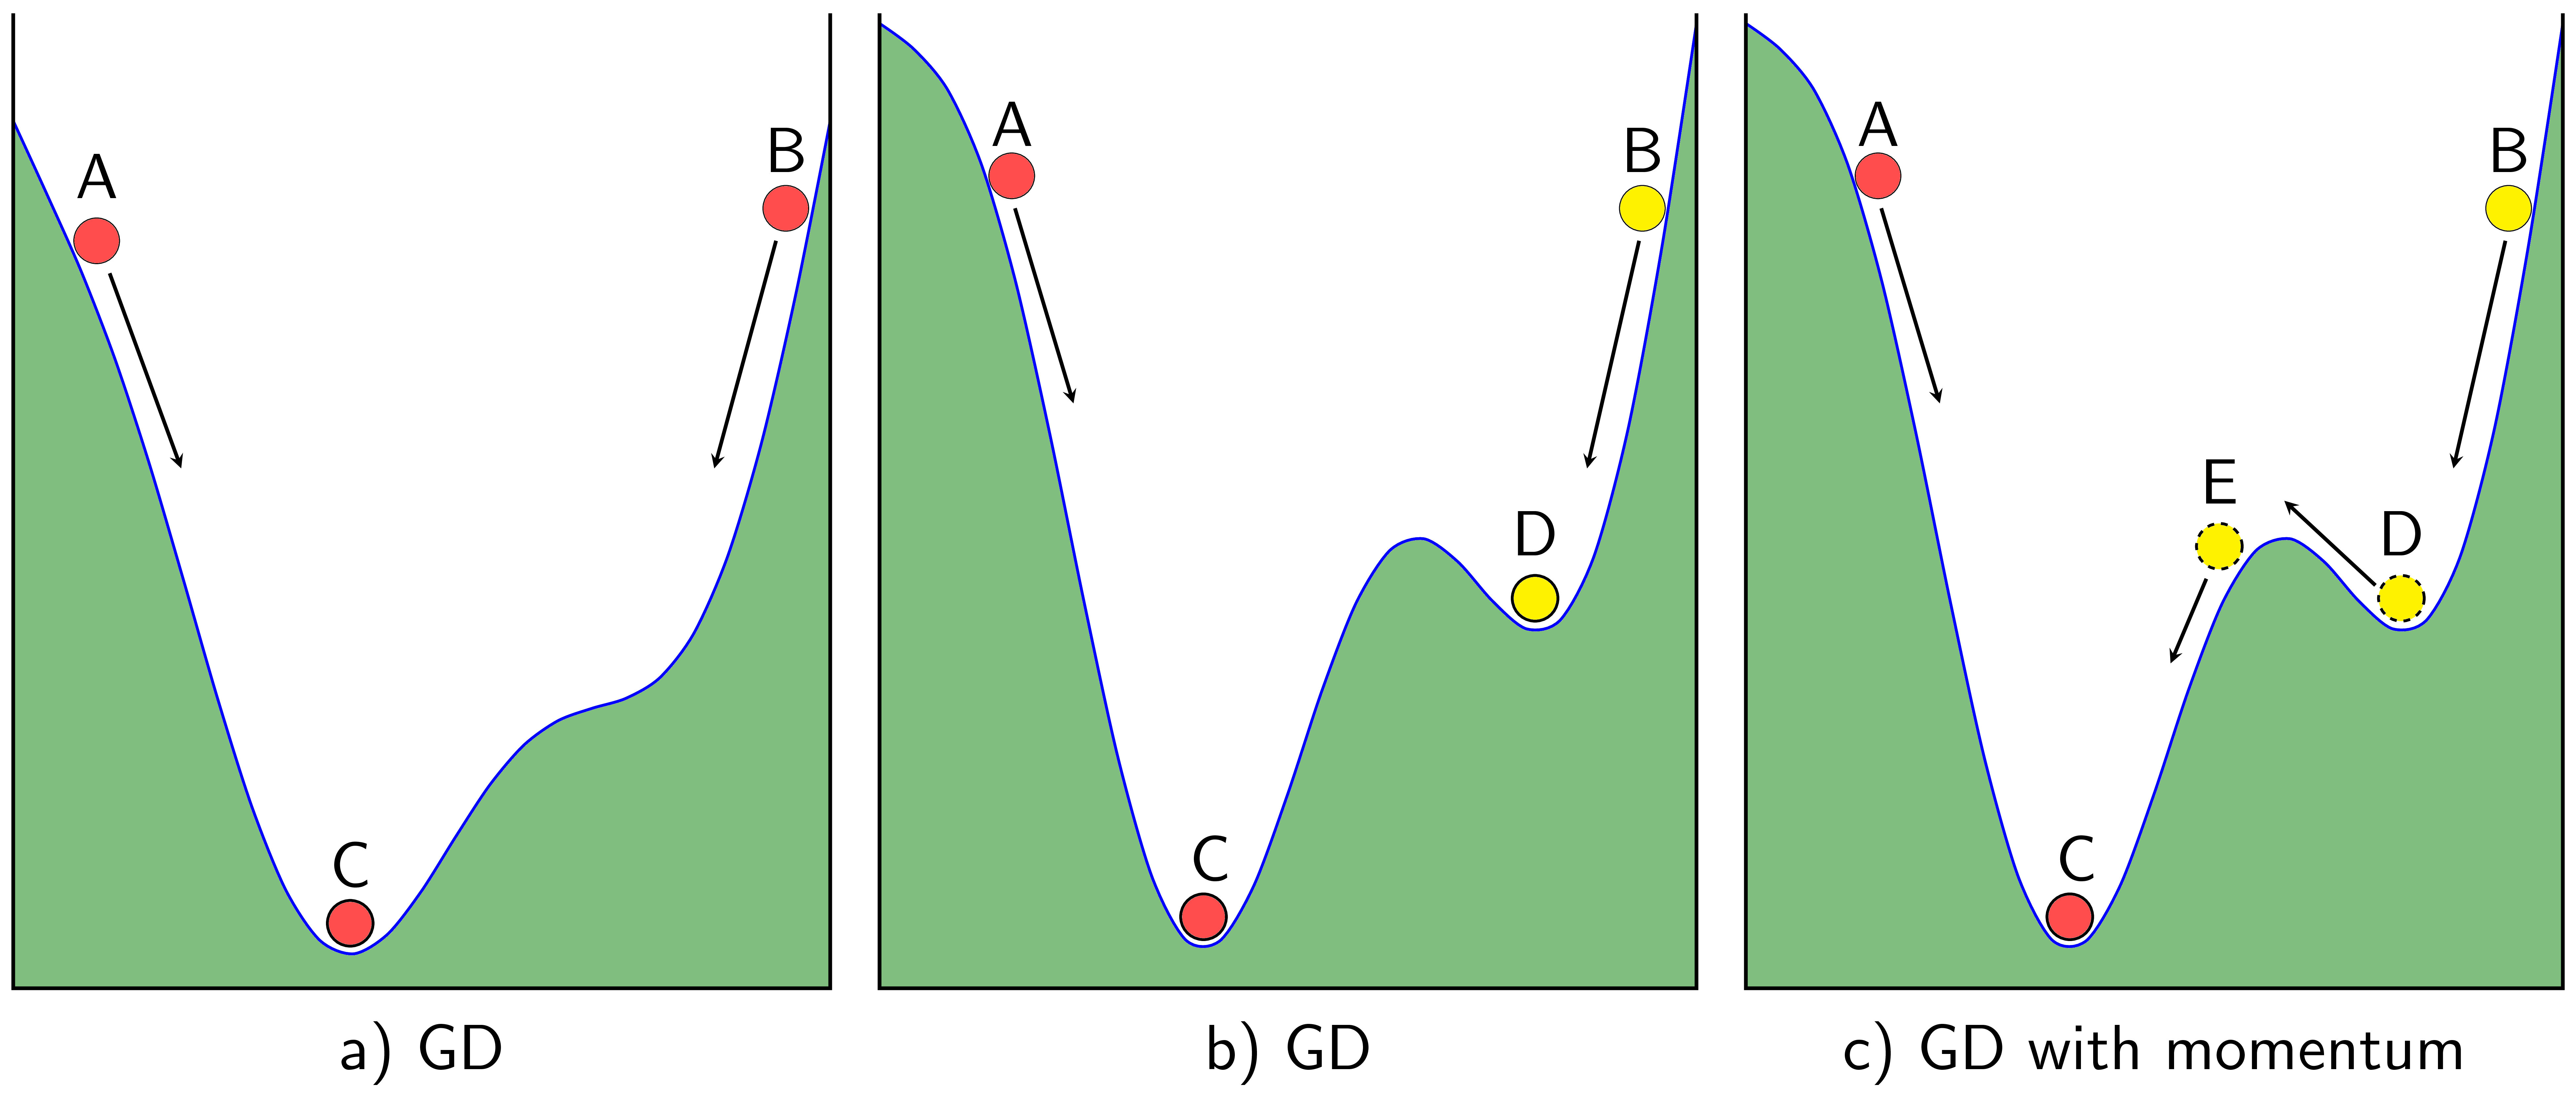
\includegraphics[scale=0.06]{chap4/c4_figs/momentum.png}
\end{center}
\caption{So sánh Gradient Descent với các hiện tượng vật lý (Nguồn: "Machine learning cơ bản" - Vũ Hữu Tiệp)}
\label{fig:gradient}
\end{figure}
\FloatBarrier

Tuy nhiên, nếu như bề mặt có hai đáy thung lũng như Hình \ref{fig:gradient}b thì tùy vào việc đặt bi ở A hay B, vị trí cuối cùng của bi sẽ ở C hoặc D. Điểm D là một điểm local minimum chúng ta không mong muốn.

Nếu suy nghĩ một cách vật lý hơn, vẫn trong Hình \ref{fig:gradient}b, nếu vận tốc ban đầu của bi khi ở điểm B đủ lớn, khi bi lăn đến điểm D, theo đà, bi có thể tiếp tục di chuyển lên dốc phía bên trái của D. Và nếu giả sử vận tốc ban đầu lớn hơn nữa, bi có thể vượt dốc tới điểm E rồi lăn xuống C như trong Hình \ref{fig:gradient}c. Đây chính là điều chúng ta mong muốn.

\subsection{Stochastic Gradient Descent}
Trong thuật toán này, tại 1 thời điểm, ta chỉ tính đạo hàm của hàm mất mát dựa trên chỉ một điểm dữ liệu $\mathbf{x_i}$ rồi cập nhật 
$\theta$ dựa trên đạo hàm này. Việc này được thực hiện với từng điểm trên toàn bộ dữ liệu, sau đó lặp lại quá trình trên. Thuật toán rất đơn giản này trên thực tế lại làm việc rất hiệu quả.

Mỗi lần duyệt một lượt qua tất cả các điểm trên toàn bộ dữ liệu được gọi là một epoch. Với GD thông thường thì mỗi epoch ứng với 1 lần cập nhật $\theta$, với SGD thì mỗi epoch ứng với $\mathbf{N}$ lần cập nhật $\mathbf{\theta}$ với $\mathbf{N}$ là số điểm dữ liệu. Nhìn vào một mặt, việc cập nhật từng điểm một như thế này có thể làm giảm đi tốc độ thực hiện 1 epoch. Nhưng nhìn vào một mặt khác, SGD chỉ yêu cầu một lượng epoch rất nhỏ (thường là 10 cho lần đầu tiên, sau đó khi có dữ liệu mới thì chỉ cần chạy dưới một epoch là đã có nghiệm tốt). Vì vậy SGD phù hợp với các bài toán có lượng cơ sở dữ liệu lớn (chủ yếu là Deep Learning mà chúng ta sẽ thấy trong phần sau của blog) và các bài toán yêu cầu mô hình thay đổi liên tục, tức online learning.

\textbf{Thứ tự lựa chọn điểm dữ liệu:}
Một điểm cần lưu ý đó là: sau mỗi epoch, chúng ta cần shuffle (xáo trộn) thứ tự của các dữ liệu để đảm bảo tính ngẫu nhiên. Việc này cũng ảnh hưởng tới hiệu năng của SGD.

Một cách toán học, quy tắc cập nhật của SGD là:
$$\theta = \theta - \eta \nabla_{\theta} J(\theta; \mathbf{x}_i; \mathbf{y}_i)$$
trong đó $J(\theta; \mathbf{x}_i; \mathbf{y}_i)$ là hàm mất mát với chỉ 1 cặp điểm dữ liệu (input, label) là $(\mathbf{x}_i, \mathbf{y}_i)$. Ngoài ra, chúng ta hoàn toàn có thể áp dụng các thuật toán tăng tốc GD như Momentum, AdaGrad,… vào SGD.

\subsection{Điều kiện dừng}
Trong thực nghiệm, có một vài phương pháp như dưới đây để xác định khi nào cần dừng số vòng lặp khi huấn luyện:
\begin{itemize}
\item Giới hạn số vòng lặp: đây là phương pháp phổ biến nhất và cũng để đảm bảo rằng chương trình chạy không quá lâu. Tuy nhiên, một nhược điểm của cách làm này là có thể thuật toán dừng lại trước khi đủ gần với nghiệm.
\item So sánh gradient của nghiệm tại hai lần cập nhật liên tiếp, khi nào giá trị này đủ nhỏ thì dừng lại. Phương pháp này cũng có một nhược điểm lớn là việc tính đạo hàm đôi khi trở nên quá phức tạp (ví dụ như khi có quá nhiều dữ liệu), nếu áp dụng phương pháp này thì coi như ta không được lợi khi sử dụng SGD và mini-batch GD.
\item So sánh giá trị của hàm mất mát của nghiệm tại hai lần cập nhật liên tiếp, khi nào giá trị này đủ nhỏ thì dừng lại. Nhược điểm của phương pháp này là nếu tại một thời điểm, đồ thị hàm số có dạng bẳng phẳng tại một khu vực nhưng khu vực đó không chứa điểm local minimum (khu vực này thường được gọi là saddle points), thuật toán cũng dừng lại trước khi đạt giá trị mong muốn.
\item Trong SGD và mini-batch GD, cách thường dùng là so sánh nghiệm sau một vài lần cập nhật.
\end{itemize}


\subsection{Áp dụng vào bài toán}
Với bộ dữ liệu của bài toán nhận dạng ngôn ngữ ký hiệu, dữ liệu là các SJM được thu thập từ trước. Dữ liệu sẽ được chia ra thành 2 tập gồm: train data (dữ liệu để huấn luyện) và test data (dữ liệu đánh giá) với tỷ lệ 80 và 20. Nghĩa là với mỗi hành động (data gồm 800 SJM) sẽ có 640 SJM để train và 160 SJM để đánh giá.
Áp dụng thuật toán SGD, với các thông số ban đầu được khởi tạo trước khi huấn luyện như sau:
\begin{itemize}
\item epoch: 50
\item learning rate: 0.01
\item
\end{itemize}
Trong quá trình huấn luyện, luận văn sử dụng phương pháp lưu lại checkpoint. Cách thức hoạt động của phương pháp này là sau mỗi epoch, accuracy trên tập test của model hiện tại được so sánh với accuracy của model trước đó. Nếu nó lớn hơn thì trọng số của mô hình sẽ được cập nhật theo trọng số mới nhất. Nếu nhỏ hơn, trọng số của mô hình trước đó vẫn được giữ lại cho đến khi accuracy khác cao hơn. Phương pháp này giúp tìm được model tối ưu nhất với accuracy cao nhất có thể.
Sau 50 epoch, ta có kết quả về độ chính xác(accuracy) và sai số (loss) trên tập train và tập test như sau:
\FloatBarrier
\begin{figure}[htp]
\begin{center}
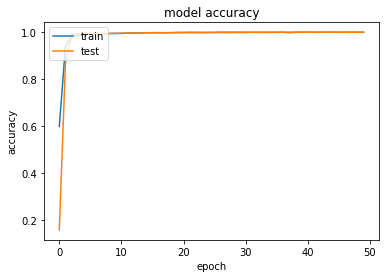
\includegraphics[scale=1]{chap4/c4_figs/train_val_acc.png}
\end{center}
\caption{Accurracy của tập train và validate}
\label{fig:pipelineS}
\end{figure}
\FloatBarrier

\FloatBarrier
\begin{figure}[htp]
\begin{center}
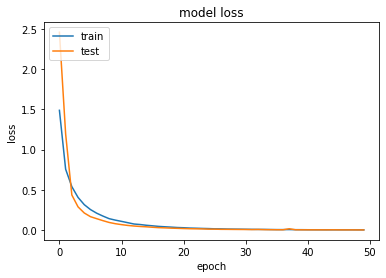
\includegraphics[scale=1]{chap4/c4_figs/train_val_l.png}
\end{center}
\caption{Loss của tập train và validate}
\label{fig:pipelineS}
\end{figure}
\FloatBarrier

Từ biểu đồ accuracy và loss của mô hình, có thể thấy mô hình đã học được rất tốt. Kể từ epoch thứ 10, mô hình đã đạt được accuracy cao và loss giảm xuống thấp. Đường biểu diễn của 2 tập đối với accuracy và loss đi sát nhau có thể phần nào dự đoán được mô hình không bị overfiting. 

\section{Kết quả}

Nhận thấy kết quả mô hình đã học được rất tốt với thuật toán này. Với kết quả cuối cùng:
\begin{itemize}
\item Train Accuracy: 1.0000
\item Test Accuracy: 0.9996
\item Train Loss: 0.0153
\item Test Loss    : 0.0123
\end{itemize}

Dựa vào những thông số trên có thể thấy kết quả sau khi huấn luyện mô hình khá tốt. Nhưng để áp dụng mô hình vào thực tế được, ta cần phải thử nghiệm và đánh giá bằng nhiều phương pháp trên tập dữ liệu mới. Chương tiếp theo sẽ trình bày về cách thức thử nghiệm, đánh giá mô hình cũng như xây dựng phần mềm ứng dụng từ mô hình. 
















